\chapter{Project}

\section{Code Concept}

In extend to this article a code base is available \footnote{\url{https://www.github.com/florianwiech/incremental-machine-learning}}.
This code base includes the reimplementation of \acrshort{ewc} and the extension of modifying the Fisher information matrix.
It uses Python 3 with the packages NumPy (version 1.16.1) and Tensorflow (version 1.13.0).
The concept documents the code structure and procedure.

The complete code consists of three files.
"main.py", "network.py" and "mnist.py".

\begin{figure}[H]
    \centering
    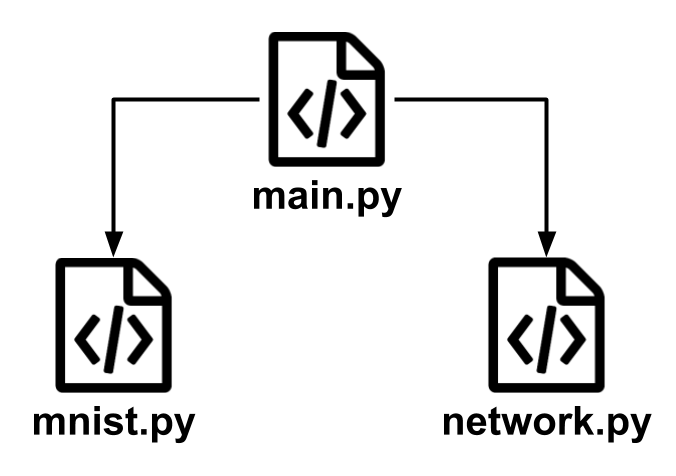
\includegraphics[scale=.4]{project/concept/files}
    \caption{File structure}
    \label{fig:concept_file_structure}
\end{figure}

The "\textbf{mnist.py}" makes the MNIST dataset available.
It loads the MNIST database automatically, reshapes the values and data structures and splits or permutes the dataset if neccesary.
After the calculation, it returns the arrays in Python standard datastructures with the extension of multi-dimensional arrays from NumPy.
\newline
"\textbf{network.py}" holds the "Network" class.
The class consists of all neccesary operations for the \acrshort{ewc} algorithm with original and adaption.
The contructor creates a neural network with 784 input neurons, three hidden layers with 800 neurons each and the ten MNIST output classes.
In addition to that, it initializes all neccesary functions like loss and accuracy.
After the initialization, the object offers several methods for training, testing and applying \acrshort{ewc} to the task.
Figure \ref{fig:concept_class_diagram} shows a class diagram of the Network class.

\begin{figure}[H]
    \centering
    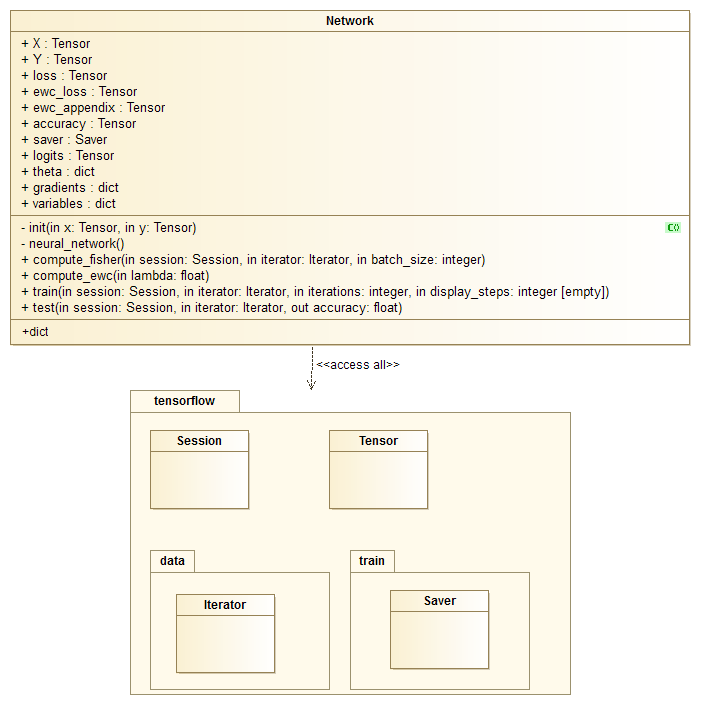
\includegraphics[scale=.6]{project/concept/class_diagram}
    \caption{Class diagram}
    \label{fig:concept_class_diagram}
\end{figure}

During execution, the network occupies multiple states.
The states distinguish if the network trains the first task or loads a previous state and retrains the network.
Figure \ref{fig:concept_state_diagram} shows the state diagram for the network:

\begin{figure}[H]
    \centering
    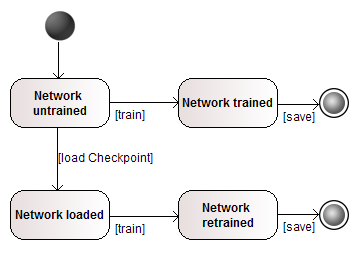
\includegraphics[scale=.8]{project/concept/state_diagram}
    \caption{State diagram}
    \label{fig:concept_state_diagram}
\end{figure}

"\textbf{main.py}" is the entrypoint of the code base.
It offers a command line tool for specification of the neccesary parameters.
\newline
The main function executes one task and saves their state in a checkpoint.
If the executed task is the first task, the network gets initialized.
In this case the \acrshort{ewc} appendix in the loss funtion is not applied.
The network gets trained, the matrix gets calculated and the final model with matrix calculation is saved in a checkpoint.
For each following ongoing task the main file has to be restarted with new args values.
In these cases the network will be initialized with the \acrshort{ewc} loss function.
The new created Tensorflow session restores a checkpoint given by the parameter (checkpoint of the task before) and the network gets retrained.

The sequential execution is shown in a sequence diagram.
The first part (Figure \ref{fig:concept_sequence_diagram_part_1}) shows the initialization of all neccesary parameters and objects.
Part 2 (Figure \ref{fig:concept_sequence_diagram_part_2}) shows the execution of training and testing the neural network.

\begin{figure}[H]
    \centering
    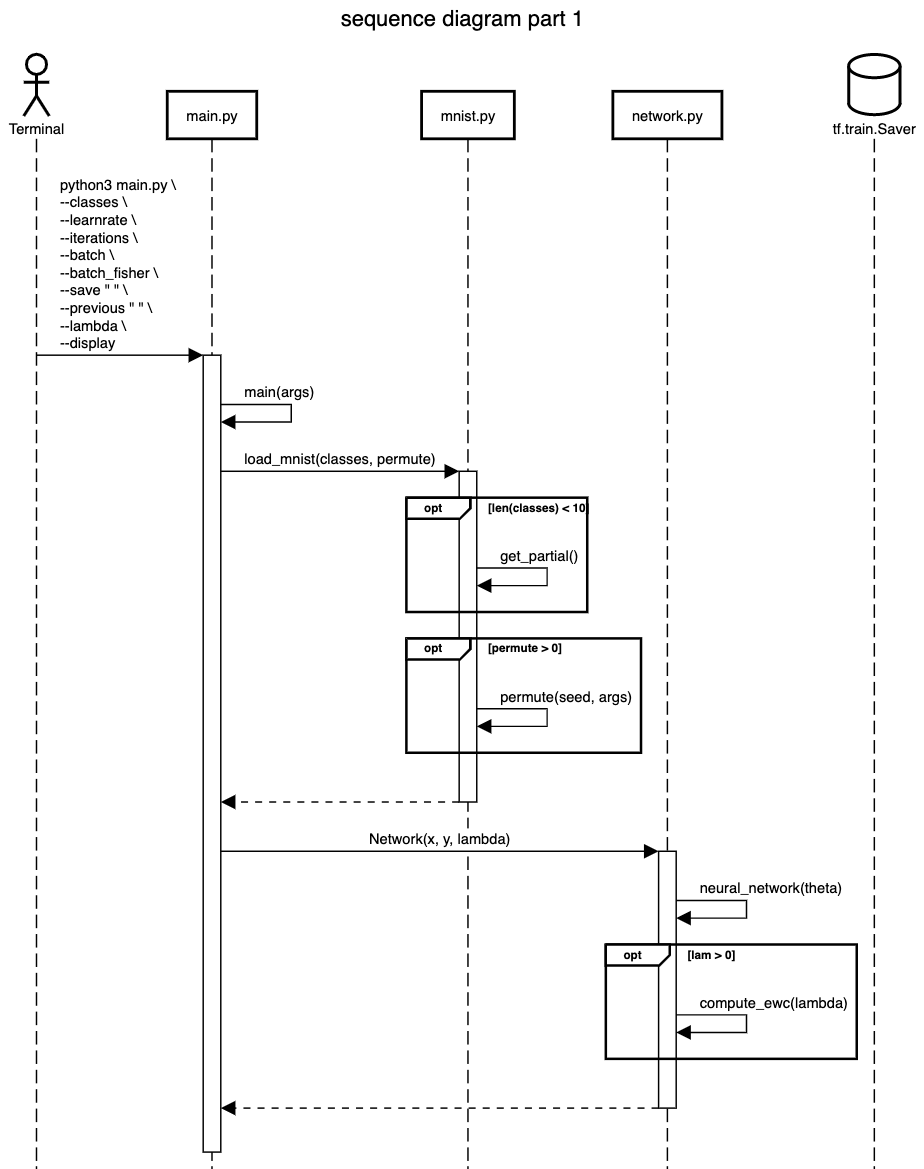
\includegraphics[width=\textwidth]{project/concept/sequence_diagram_part_1}
    \caption{Sequence diagram part 1}
    \label{fig:concept_sequence_diagram_part_1}
\end{figure}

\begin{figure}[H]
    \centering
    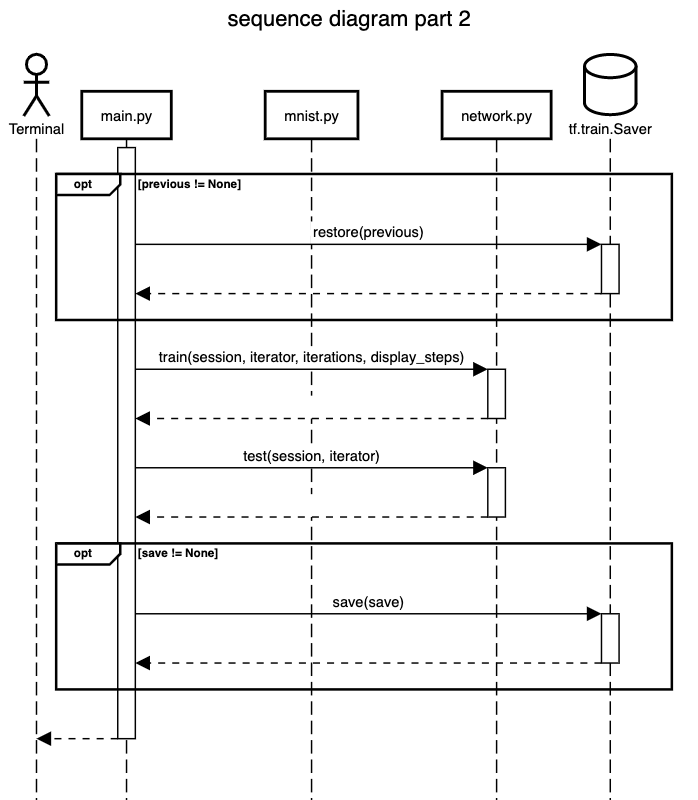
\includegraphics[width=\textwidth]{project/concept/sequence_diagram_part_2}
    \caption{Sequence diagram part 2}
    \label{fig:concept_sequence_diagram_part_2}
\end{figure}

\newpage
\section{Baseline}

Before adapting the \acrshort{ewc} algorithm, the codebase has to proof that it delivers the results of the \acrshort{ewc} paper \cite{elastic-weight-consolidation}.
The implemented \acrshort{ewc} algorithm is tested in the constructed benchmarks described in Project Goals (Section \ref{project_goals}):

\subsection{Disjoint 9-1}

In this benchmark the MNIST dataset is split into two tasks.
The first task $T_1$ includes the numbers zero to eight and the second task $T_2$ number nine.

The training of the tasks $T_1$ and $T_2$ is implemented with the following hyperparameters:

\begin{table}[H]
    \centering
    \begin{tabular}{ |l|l|l|  }
        \hline
        Task $\to$ & $T_1$ & $T_2$ \\
        \hline\hline
        samples & 54,000 & 5,900 \\
        \hline
        batch size & 100 & 100 \\
        \hline
        training iterations & 2,500 & 2,500 \\
        \hline
        learning rate & 0.001 & 0.00001 \\
        \hline
        lambda ($\lambda$) & 0 & 100,000 \\
        \hline
    \end{tabular}
    \caption{Baseline D9-1}
    \label{table:base_d91}
\end{table}

\begin{figure}[H]
    \centering
    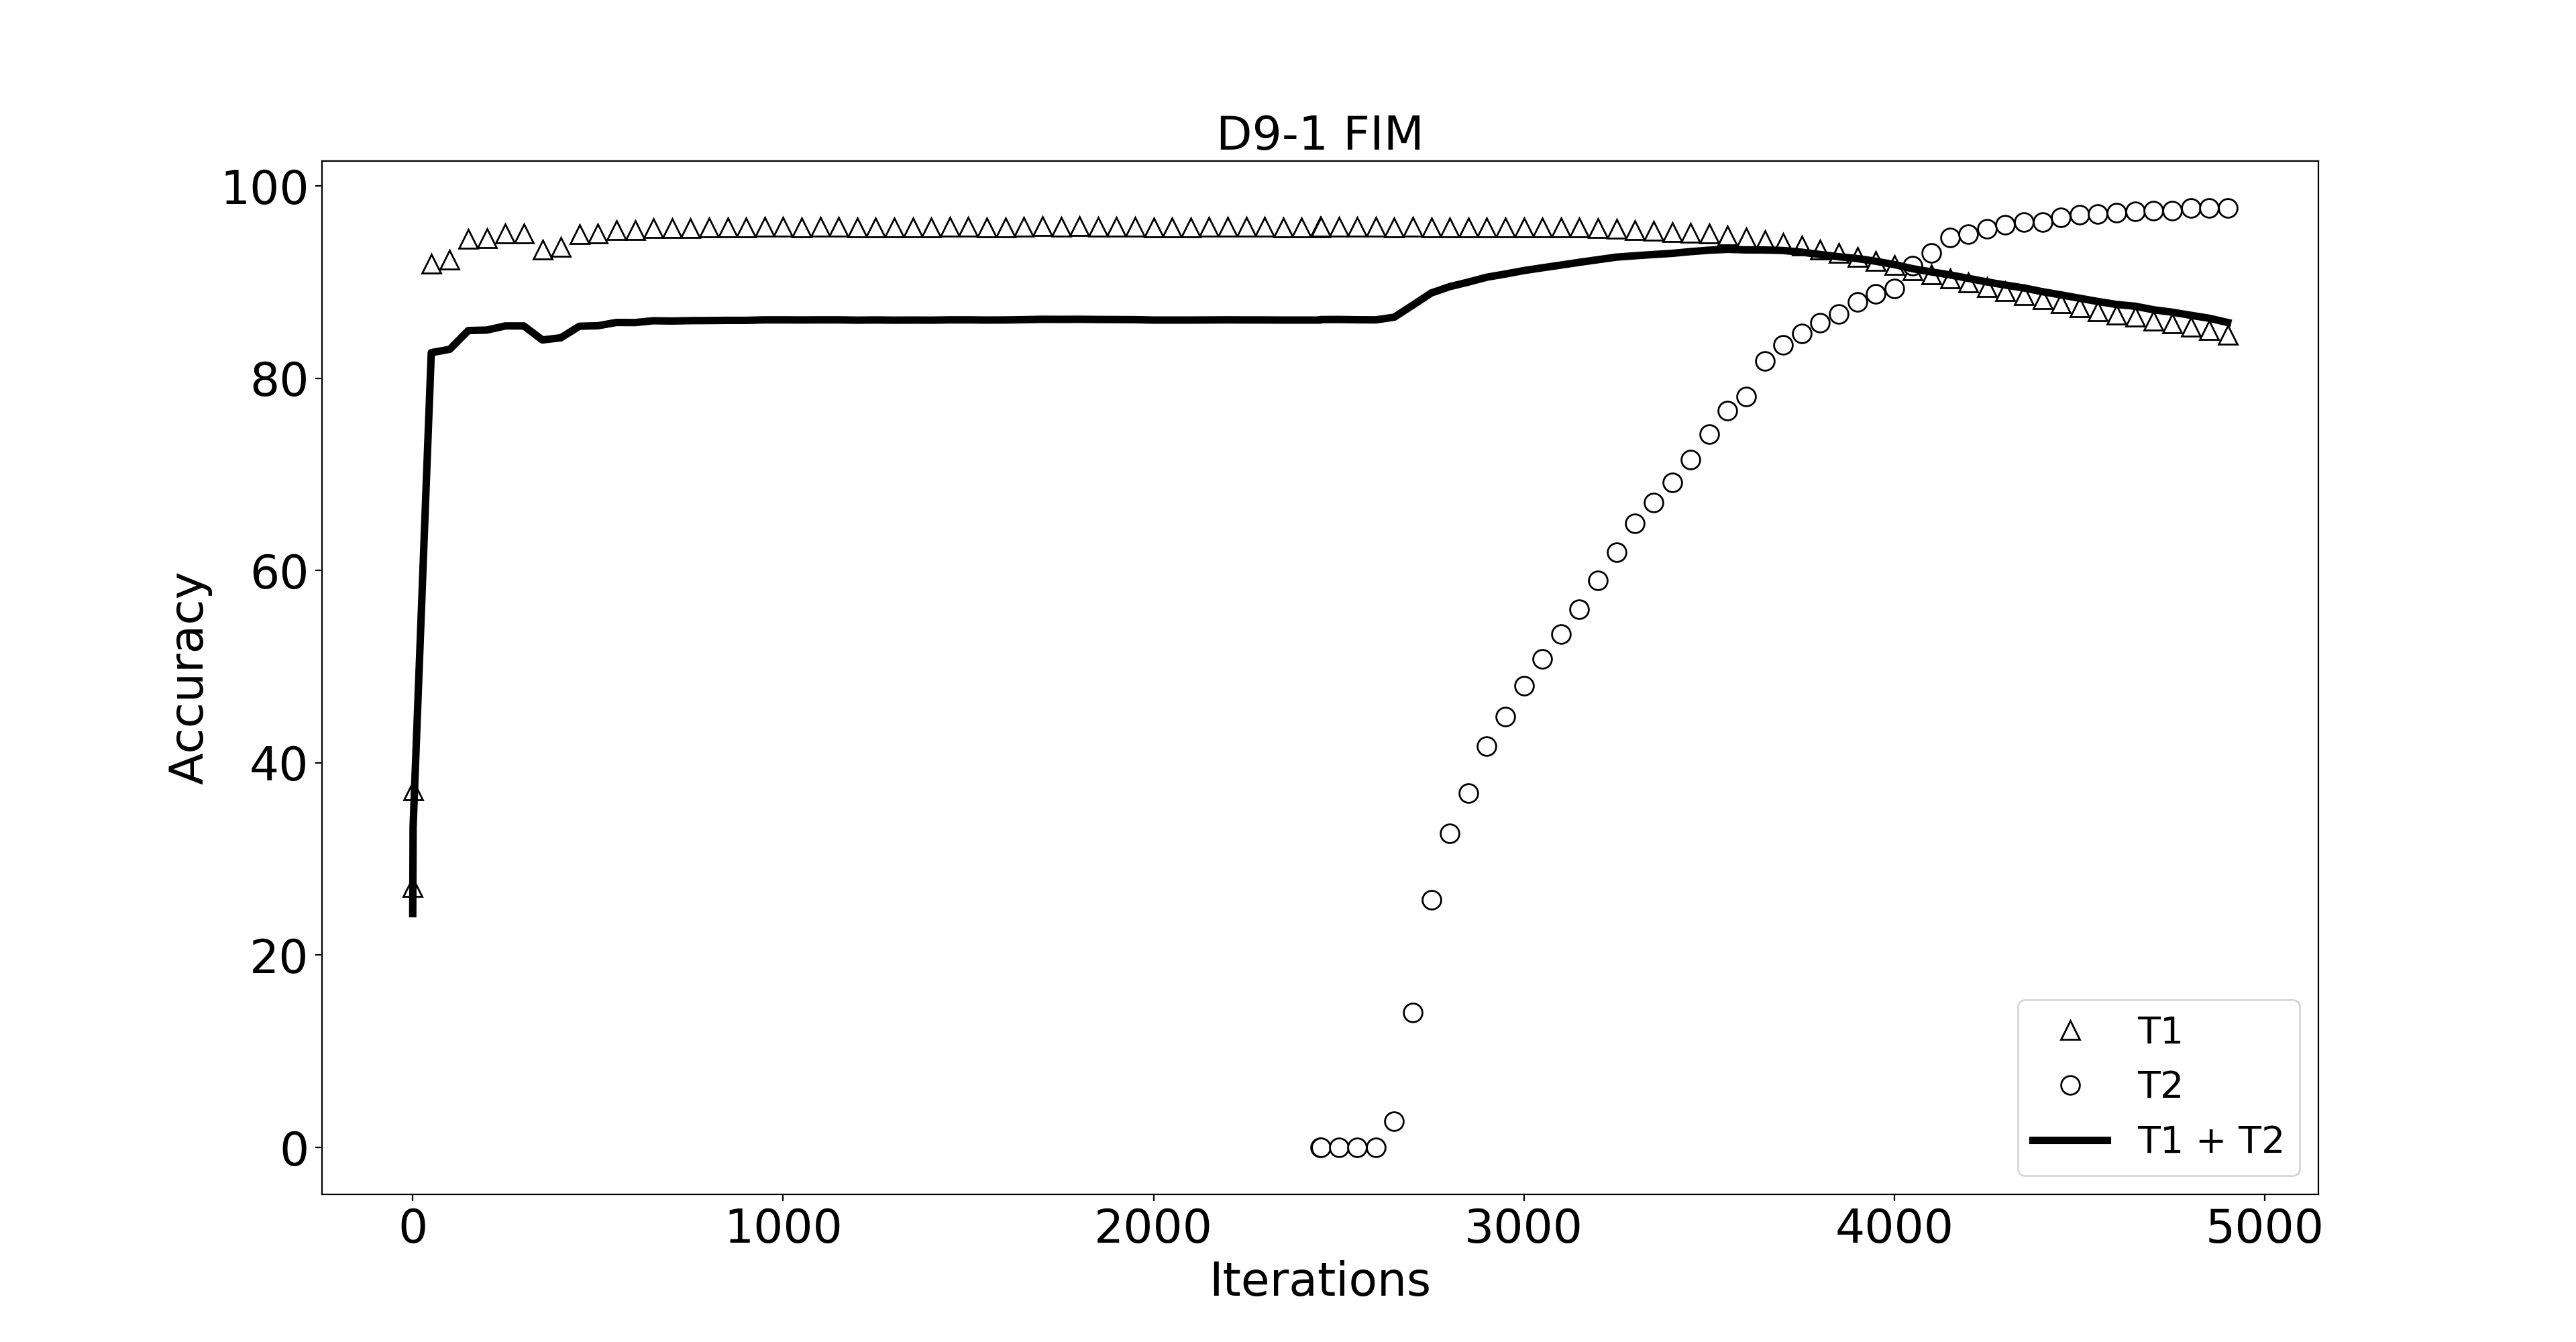
\includegraphics[width=\textwidth]{project/baseline/D91_FIM}
    \caption{\acrshort{ewc} D9-1}
    \label{fig:ewc_d9-1}
\end{figure}

Figure \ref{fig:ewc_d9-1} shows the training of task $T_1$ (white background) and re-training with task $T_2$ (gray background).
The blue line ($\triangle$) represents the accuracy on $T_1$, the red line ($\square$) on $T_2$ and the green line ($\bigcirc$) the complete dataset ($T_1 + T_2$).
After the training, $T_1$ results in 96\% accuracy.
While re-training, the complete dataset peaks at 92\% and decreases to 80\%.
Compared to the performance at the end of the training, it indicates a loss of 6\% after the re-training.
At the end of the re-training, $T_1$ is decreased to 78\% and $T_2$ measures 97\% accuracy.
\newline
This documents that the reimplementation works with sequential learning tasks that contain small amounts of data.

\subsection{Disjoint 5-5}

In this benchmark $T_1$ contains the numbers zero to four whereas $T_2$ includes the numbers five to nine.

The training of the tasks $T_1$ and $T_2$ is implemented with the following hyperparameters:

\begin{table}[H]
    \centering
    \begin{tabular}{ |l|l|l|  }
        \hline
        Task $\to$ & $T_1$ & $T_2$ \\
        \hline\hline
        samples & 30,500 & 29,400 \\
        \hline
        batch size & 100 & 100 \\
        \hline
        training iterations & 2,500 & 2,500 \\
        \hline
        learning rate & 0.001 & 0.00001 \\
        \hline
        lambda ($\lambda$) & 0 & 100,000 \\
        \hline
    \end{tabular}
    \caption{Baseline D5-5}
    \label{table:base_d55}
\end{table}

\begin{figure}[H]
    \centering
    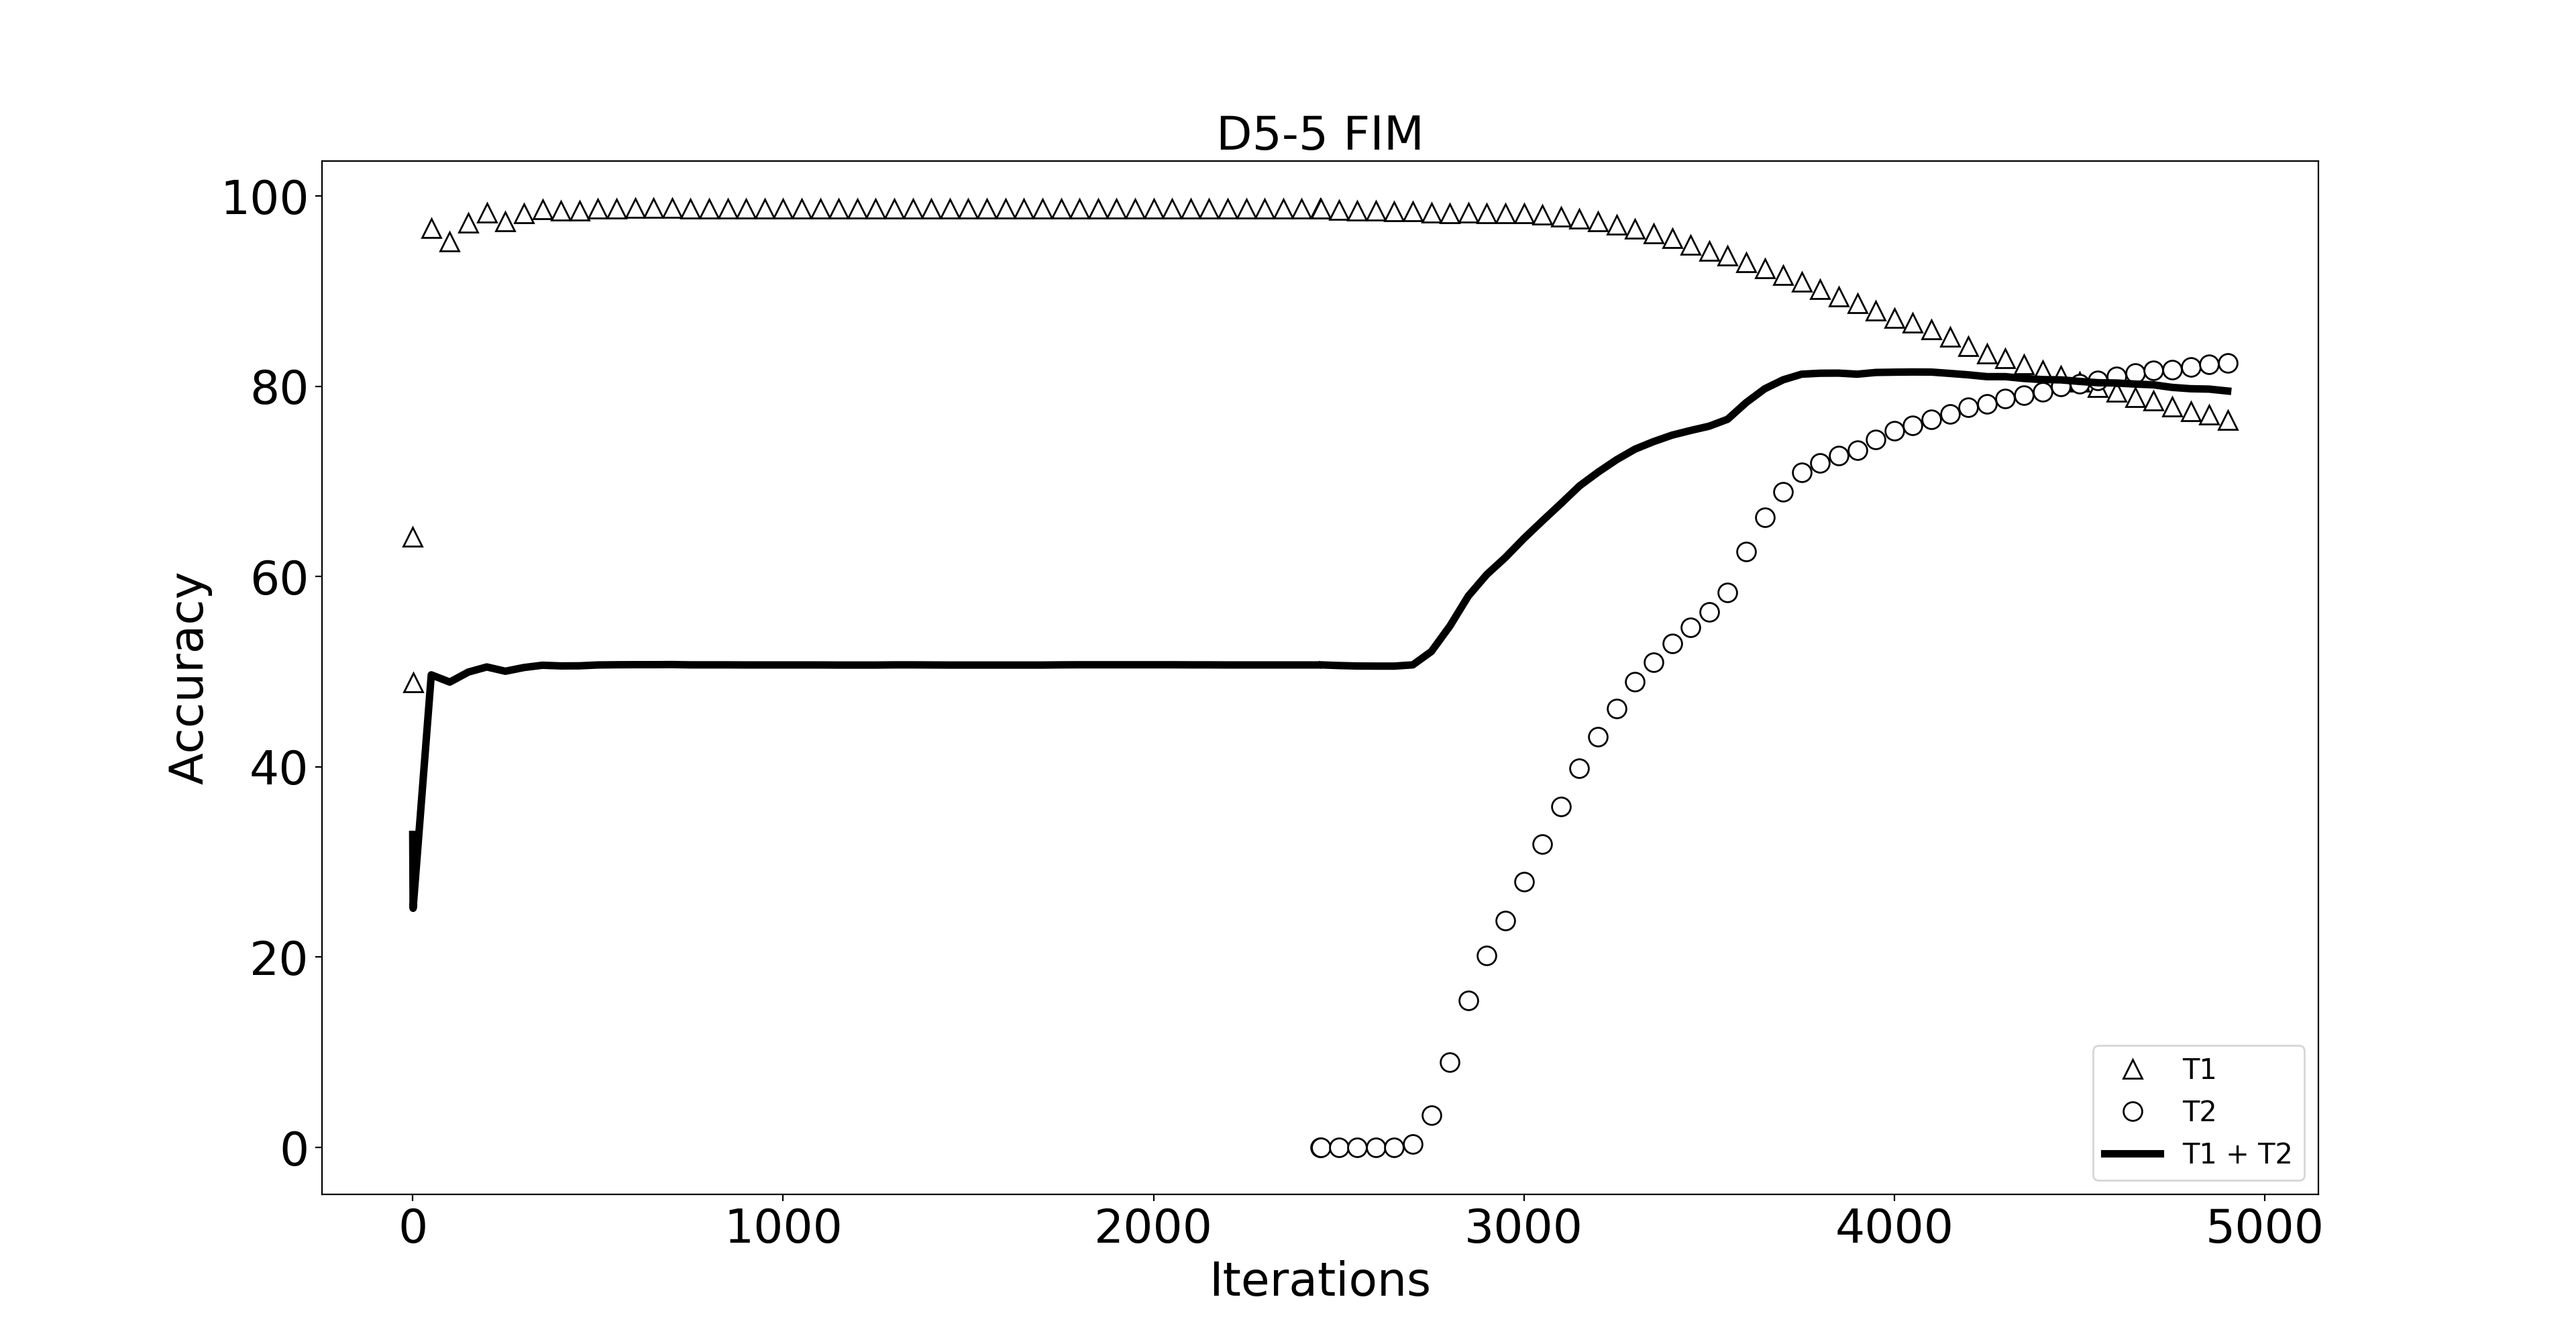
\includegraphics[width=\textwidth]{project/baseline/D55_FIM}
    \caption{\acrshort{ewc} D5-5}
    \label{fig:ewc_d5-5}
\end{figure}

Figure \ref{fig:ewc_d5-5} shows the training of task $T_1$ (white background) and re-training with task $T_2$ (gray background).
The blue line ($\triangle$) represents the accuracy on $T_1$, the red line ($\square$) on $T_2$ and the green line ($\bigcirc$) the complete dataset ($T_1 + T_2$).
After the training, $T_1$ results in 99\% accuracy.
While re-training, the complete dataset increases its accuracy from 51\% to 81\%.
At the end of the re-training, $T_1$ is decreased to 80\% and $T_2$ measures 81\% accuracy.
\newline
It shows that the reimplementation of the \acrshort{ewc} algorithm works.
Catastrophic forgetting is reduced in the re-training of an approximately equally task.

\subsection{Permuted 10-10}

This benchmark uses the complete MNIST dataset in the first task $T_1$ and permutes the complete dataset for the second task $T_2$.
Figure \ref{fig:intro_mnist_permuted_example} shows a MNIST picture with the number zero and its permutation.

The training of the tasks $T_1$ and $T_2$ is implemented with the following hyperparameters:

\begin{table}[H]
    \centering
    \begin{tabular}{ |l|l|l| }
        \hline
        Task $\to$ & $T_1$ & $T_2$ \\
        \hline\hline
        samples & 60,000 & 60,000 \\
        \hline
        permutation seed & - & 0 \\
        \hline
        batch size & 100 & 100 \\
        \hline
        training iterations & 2,500 & 20,000 \\
        \hline
        learning rate & 0.001 & 0.00001 \\
        \hline
        lambda ($\lambda$) & 0 & 100,000 \\
        \hline
    \end{tabular}
    \caption{Baseline P10-10}
    \label{table:base_p1010}
\end{table}

\begin{figure}[H]
    \centering
    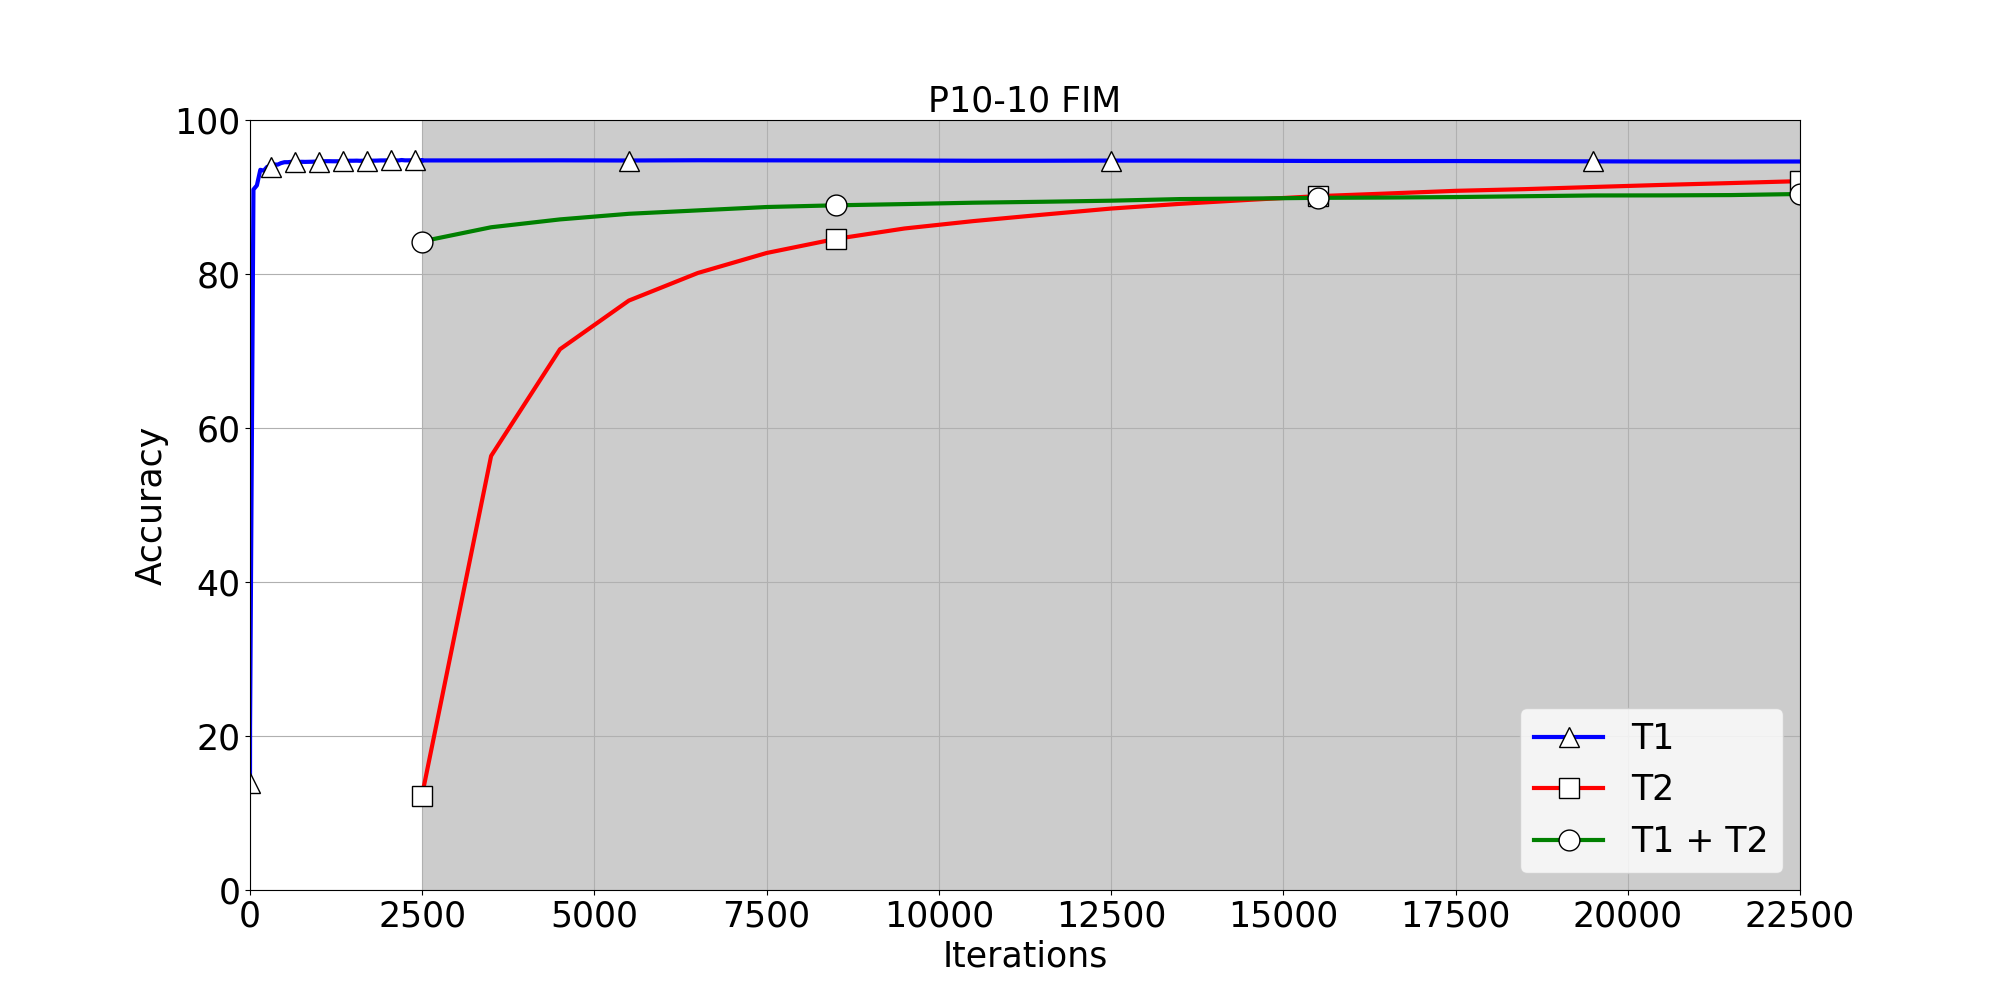
\includegraphics[width=\textwidth]{project/baseline/PM_FIM}
    \caption{\acrshort{ewc} P10-10}
    \label{fig:ewc_p10-10}
\end{figure}

Figure \ref{fig:ewc_p10-10} shows the training of task $T_1$ (white background) and re-training with task $T_2$ (gray background).
The blue line ($\triangle$) represents the accuracy on $T_1$, the red line ($\square$) on $T_2$ and the green line ($\bigcirc$) the complete dataset ($T_1 + T_2$).
After the training, $T_1$ results in 95\% accuracy.
The complete dataset starts with 84\% accuracy into the re-training.
It is able to gain 6\% and quantifies 90\% accuracy at the end of the re-training.
$T_1$ still measures 95\% accuracy and $T_2$ amounts 92\% accuracy.
\newline
The reimplementation is able to learn different data from the same classes, as shown in the EWC paper \cite{elastic-weight-consolidation} (Figure \ref{fig:ewc_permuted_example}).

\newpage

\section{Critical review of \acrshort{ewc} and improvements}
\label{project_review_improvements}

The \acrshort{ewc} loss function uses the original loss function with the \acrshort{ewc} appendix:

\begin{equation}
    \mathcal{L} = 
    \mathcal{L}^{CE} 
    + \sum_{i} 
        \frac{\lambda}{2} 
        F_{i} 
        (\theta_{i} - \theta_{T_1,i}^{*})^2
\end{equation}

For a better understanding the abstract parameter $\theta$ can be split into the explicit weight and bias parameters.
The weights are represented as $W^i$ matrices and the biases as $B^i$ vectors.
The index $i$ stands for each layer, $i \in \{ 0, \dots, L-1 \}$.

The \acrshort{ewc} term has the following notation:

\begin{equation}
    \begin{split}
        \mathcal{L} = \mathcal{L}^{CE}
        & + \frac{\lambda}{2} \sum_{i=0}^{L-1} \sum_{k, l} F_{k, l}^{W^i}\left(W^i_{k, l}-W^{i,{T_1}}_{k, l} \right)^2
        \\
        & +  \frac{\lambda}{2}\sum_{i=0}^{L-1} \sum_{k}F^{B^i}_k\left(B^i_{k}-B^{i,{T_1}}_{k} \right)^2
    \end{split}
\end{equation}

As proposed in Elastic Weight Consolidation (Section \ref{foundation_ewc}, \cite{elastic-weight-consolidation}) the authors use the Fisher information matrix for the loss calculation.
The Formula \ref{eq:original_fisher} shows the \acrshort{fim}.
$N$ represents the training samples, $\mathcal{L}$ the loss functions and $\theta$ the set of weight matrices and bias vectors:

\begin{equation}
    F_{ij} = 
    \frac{1}{N} 
    \sum_{n=1}^{N} 
    \left(
        \frac{\partial \mathcal{L} \left( x_n \right) }{\partial \theta_{i}} 
        \cdot 
        \frac{\partial \mathcal{L} \left( x_n \right) }{\partial \theta_{j}}
    \right)
    \label{eq:original_fisher}
\end{equation}

In fact, they only use the diagonal of the Fisher information matrix:

\begin{equation}
    \begin{split}
        \vec{F} & = diag \left( F_{ij} \right)
        \\
        F_{j} & = 
        \frac{1}{N} 
        \sum_{n=1}^{N} 
        \left(
            \frac{\partial \mathcal{L} \left( x_n \right) }{\partial \theta_{j}}
        \right)^2
    \end{split}
    \label{eq:ewc_diagonal_fisher}
\end{equation}

As well as the \acrshort{ewc} term, this matrix can be split into the weight matrices and the bias vectors:

\begin{equation}
    \begin{split}
        F^{W^i}_{j,k} & = 
        \frac{1}{N} 
        \sum_{n=1}^{N} 
        \left(
            \frac{\partial \mathcal{L} \left( x_n \right) }{\partial W^i_{j,k}}
        \right)^2
        \\
        \vec{F}^{B^i}_j & = 
        \frac{1}{N} 
        \sum_{n=1}^{N} 
        \left(
            \frac{\partial \mathcal{L} \left( x_n \right) }{\partial B^i_{j}}
        \right)^2
    \end{split}
\end{equation}

% structure for understandability
The reports \cite{better-weight-consolidation,elastic-weight-consolidation} justify that assuming the \acrshort{fim} is diagonal is common practice \cite{elastic-weight-consolidation,better-weight-consolidation,incremental-moment-matching}.
The assumption, \acrshort{fim} being diagonal, reduces the operations from $O(N^2)$ to $O(N)$ \cite{elastic-weight-consolidation,better-weight-consolidation}.
$N$ is the number of elements in $\theta$ \cite{elastic-weight-consolidation,better-weight-consolidation}.
Because of that, matrices - even large ones - are calculated much faster \cite{elastic-weight-consolidation,better-weight-consolidation}.
In general, this assumption receives rather promising results. % in use with the algorithm
\cite{elastic-weight-consolidation,incremental-moment-matching}.

It seems that the rather promising results are the main justification for using only the diagonal of the \acrshort{fim}.
\newline
This article describes another calculation of the \acrshort{ewc} loss.
This time the \acrshort{ewc} loss is not based on diagonal assumptions, but instead on a mathematical principle.
\newline
A closer look to the \acrshort{ewc} appendix shows, that the term $(\theta_i - \theta^*_{T_1,i})^2$ calculates the divergence between the new calculated parameters and the parameters of the previously learned task.
The square is used to receive only positive values.
\newline
The original algorithm uses the diagonal \acrshort{fim}, which shows the importance of the parameters.
By multiplying the diagonal \acrshort{fim} with the calculated divergence, the algorithm knows, which parameters should be protected.
\newline
% In contrast to that, this time, a new way to measure the important parameters is needed.
% TODO formulation
In contrast to that, this time, the first derivative of the loss $\mathcal{L}$ according to the parameters is used to measure the importance of the parameters.
The first derivative of the loss $\mathcal{L}$ according to the parameters is its slope.
Network adjustments alter the parameters with high gradients significantly compared to the parameters with lower gradients.
By changing parameters with higher gradients, the network balance is destroyed faster.
This is why parameters with high gradients are more important than the ones with lower gradients.

Formula \ref{eq:loss_with_derivative} shows the loss function and its first derivative according to the parameters $\theta$. $N$ represents the training samples.

\begin{equation}
    \begin{split}
        \mathcal{L}_k & = 
        \frac{1}{N}
        \sum_{n} 
            \mathcal{L}(x_n)
        \\
        \frac{\partial \mathcal{L}(x_n)}{\partial \theta_k} & = 
        \frac{1}{N}
        \sum_{n} 
            \frac{\partial \mathcal{L}(x_n)}{\partial \theta_k}
    \end{split}
    \label{eq:loss_with_derivative}
\end{equation}

The first derivative gets squared in order to receive positive and higher values.
The operation is allowed because it does not change the difference of the values, which is the important factor.

\begin{equation}
    \left[
        \frac{\partial \mathcal{L}(x_n)}{\partial \theta_k}
        \right]^2
    = 
    \left[
        \frac{1}{N}
        \sum_{n} 
            \frac{\partial \mathcal{L}(x_n)}{\partial \theta_k}
        \right]^2
\end{equation}

Equation \eqref{eq:gradient_matrix} shows the new approach. $N$ represent the training samples.

\begin{equation}
    \mathcal{F}_k =
    \left(
        \frac{1}{N}
        \sum_{n} 
            \frac{\partial \mathcal{L}(x_n)}{\partial \theta_k}
        \right)^2
    \label{eq:gradient_matrix}
\end{equation}

Since $\theta$ only consists of weight matrices and bias vectors, it can be re-arranged as illustrated:

\begin{equation}
    \begin{split}
        F^{W^i}_{j,k} & = 
        \left(
            \frac{1}{N} 
            \sum_{n=1}^{N}
            \frac{\partial \mathcal{L} \left( x_n \right) }{\partial W^i_{j,k}}
        \right)^2
        \\
        \vec{F}^{B^i}_j & = 
        \left(
            \frac{1}{N} 
            \sum_{n=1}^{N} 
            \frac{\partial \mathcal{L} \left( x_n \right) }{\partial B^i_{j}}
        \right)^2
    \end{split}
\end{equation}

The new approach is termed as \acrfull{gm}.
\newline
The comparison of Formula \ref{eq:ewc_diagonal_fisher} and Formula \ref{eq:gradient_matrix} points out, that both formulas are quite similar.
Both compute the expectation values over loss gradients.
\newline
The \acrshort{fim} specifies to square the gradient of every sample.
Since, it is common practice to use mini-batches, the gradients are summed up over the mini-batch and averaged at the end of the training step.
By contrast, the \acrlong{gm} squares the gradient of every mini-batch.
\newline
In the case of $N=1$ they are equivalent.

The current reference implementation \footnote[1]{\url{https://github.com/ariseff/overcoming-catastrophic}} of \acrshort{ewc} uses Tensorflow.
A problem by calculating the \acrshort{fim} in Tensorflow is that it is neccesary to get the gradients for every sample but Tensorflow does not expose them.
That is why the reference implementation builds a complex workaround by hardcoding the gradients directly into the computation graph of Tensorflow.
This increases the memory consumption by the batch size.
The computation of a full batch would directly run out of memory.
As a consequence the developer sets the batch size for this computation to the fixed rate of 100.
In Contrast, the \acrlong{gm} squares the gradients, which solve the problem.
\cite{github_ewc_issue_one}

The following section tests the \acrlong{gm} on the D9-1, D5-5 and P10-10 benchmarks.

\newpage
\section{Experimental Results}

This following section shows the results of \acrshort{ewc} with the Gradient matrix.
It tests several parameter values.
Mainly the learning rate and lambda are varied.
The network features are listed in Section \ref{foundations_deep_neural_network}.

\subsection{Disjoint 9-1}

In this experiment the MNIST dataset is split into two tasks.
The first task $T_1$ includes the numbers zero to eight and the second task $T_2$ number nine.

The training of the tasks $T_1$ and $T_2$ is implemented with the following hyperparameters:

\begin{table}[H]
    \centering
    \begin{tabular}{ |l|l|l|  }
        \hline
        Task $\to$ & $T_1$ & $T_2$ \\
        \hline\hline
        samples & 54,000 & 5,900 \\
        \hline
        training batch size & 100 & 100 \\
        \hline
        training iterations & 2,500 & 2,500 \\
        \hline
        learning rate & 0.001 & 0.00001 \\
        \hline
        \acrshort{gm} batch size & 1,000 & - \\
        \hline
        lambda ($\lambda$) & 0 & 100,000 \\
        \hline
    \end{tabular}
    \caption{Experiment D9-1 parameters}
    \label{table:exp_d91_params}
\end{table}

\begin{figure}[H]
    \centering
    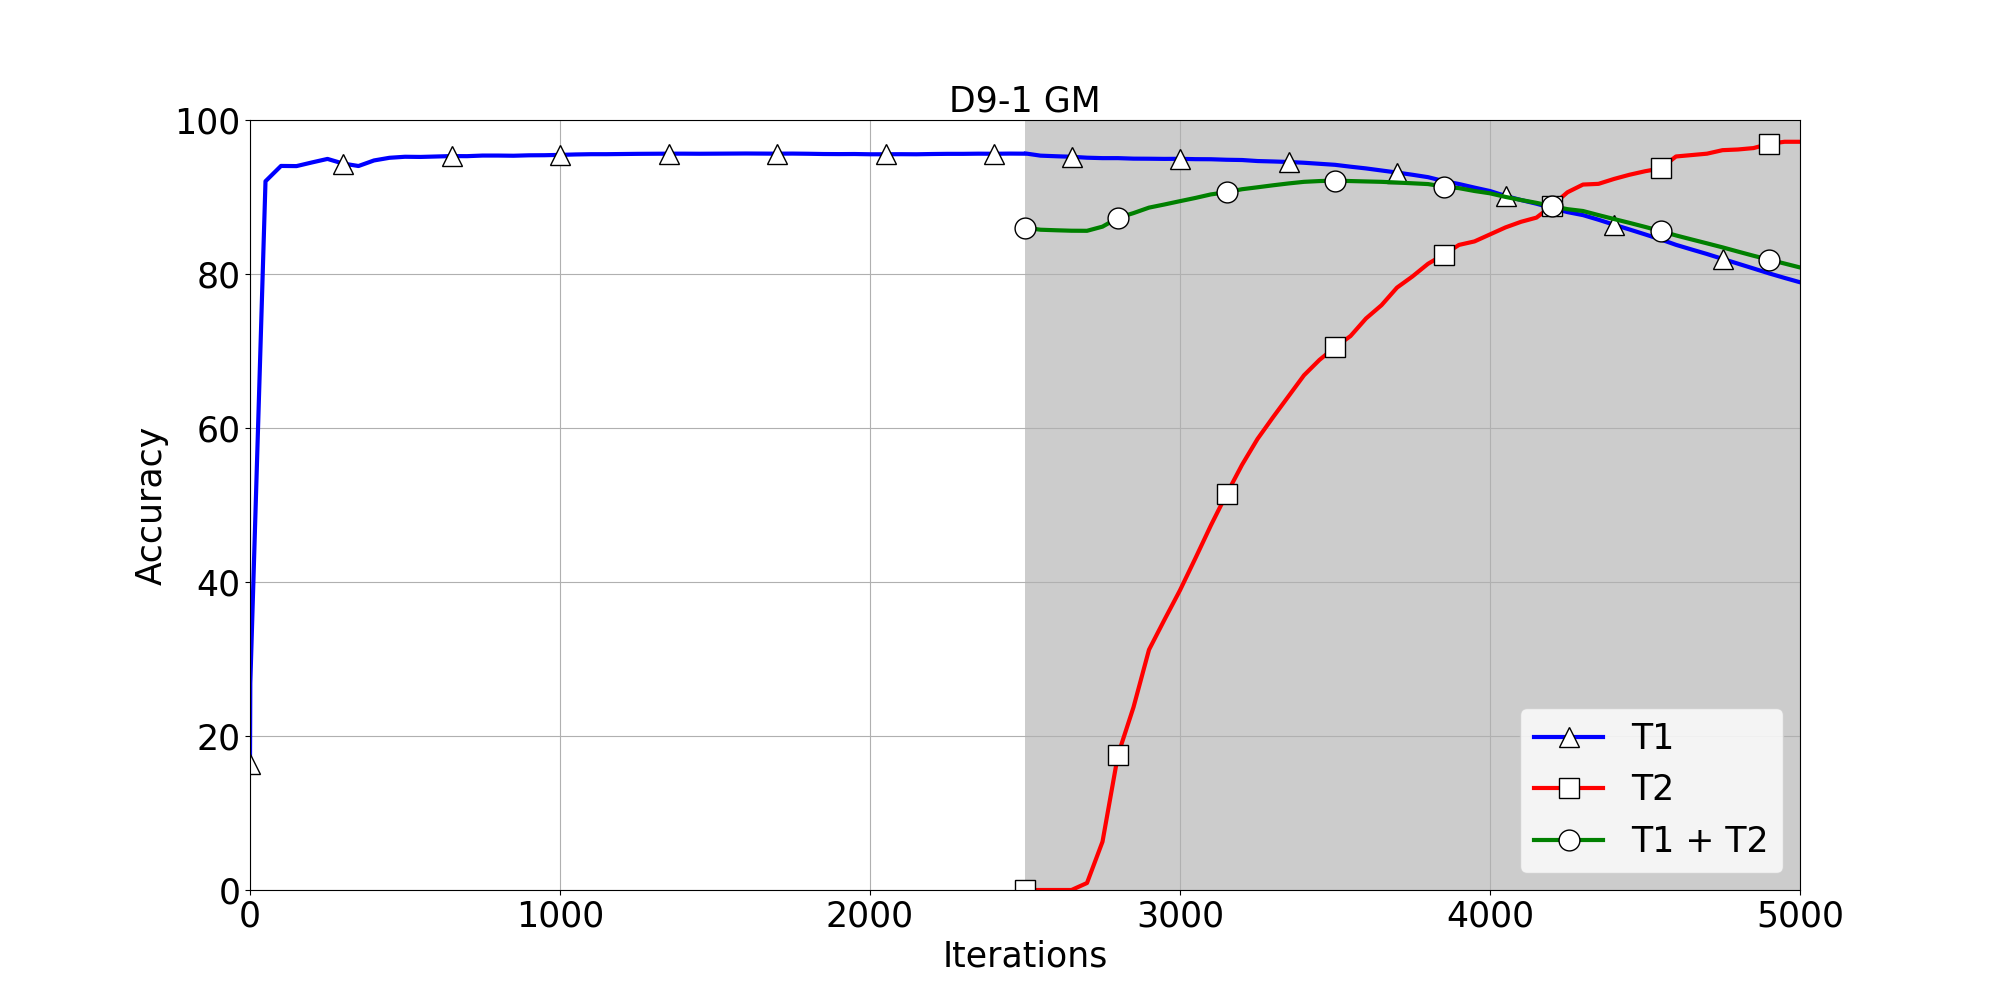
\includegraphics[width=\textwidth]{project/experiments/D91_GM}
    \caption{Experiment D9-1}
    \label{fig:exp_d9-1_bs1k}
\end{figure}

Figure \ref{fig:exp_d9-1_bs1k} shows the training of task $T_1$ (white background) and re-training with task $T_2$ (gray background).
The blue line ($\triangle$) represents the accuracy on $T_1$, the red line ($\square$) on $T_2$ and the green line ($\bigcirc$) the complete dataset ($T_1 + T_2$).
After the training, $T_1$ results in 96\% accuracy.
While re-training, the complete dataset peaks at 92\% and decreases to 81\%.
Compared to the performance at the end of the training, it indicates a loss of 5\% after the re-training.
At the end of the re-training, $T_1$ is decreased to 79\% and $T_2$ measures 97\% accuracy.
\newline
It indicates, that the \acrshort{ewc} algorithm with the Gradient matrix is capable of learning small amounts of data.
However, it exhibits a significant sacrifice.

\begin{table}[H]
    \centering
    \begin{tabular}{ |c|l|l|l|  }
        \hline
        \multicolumn{2}{|c|}{parameters} & \multicolumn{2}{c|}{accuracy after $T_2$ training} \\
        \hline
        learning rate & lambda & $T_2$ & complete dataset\\
        \hline
        \hline
        \multirow{6}{*}{0.001} & 1,000 & 100\% & 11.20\%\\
                            & 10,000 & 100\% & 12.78\%\\
                            & 100,000 & 100\% & 12.93\% \\
                            & 1,000,000 & 100\% & 15.92\% \\
                            & 1,010,000 & 100\% & 15.14\% \\
                            & 1,050,000 & 100\% & 14.65\% \\
        \hline
        \multirow{6}{*}{0.0001} & 1,000 & 100\% & 42.22\%\\
                                & 10,000 & 100\% & 40.47\%\\
                                & 100,000 & 100\% & 37.86\% \\
                                & 1,000,000 & 100\% & 41.99\% \\
                                & 1,010,000 & 100\% & 40.09\% \\
                                & 1,050,000 & 100\% & 40.11\% \\
        \hline
        \multirow{6}{*}{0.00001} & 1,000 & 98.91\% & 82.62\%\\
                                & 10,000 & 98.82\% & 83.48\%\\
                                & 100,000 & 97.82\% & 85.41\% \\
                                & 1,000,000 & 87.78\% & 90.84\% \\
                                & 1,010,000 & 87.69\% & 90.86\% \\
                                & 1,050,000 & 87.51\% & 90.87\% \\
        \hline
        \multirow{6}{*}{0.000001} & 1,000 & 94.27\% & 90.2\% \\
                                & 10,000 & 80.34\% & 92.81\% \\
                                & 100,000 & 3.18\% & 86.4\% \\
                                & 1,000,000 & 0.0\% & 86.17\% \\
                                & 1,010,000 & 0.0\% & 86.16\% \\
                                & 1,050,000 & 0.0\% & 86.16\% \\
        \hline
    \end{tabular}
    \caption{Experiment D9-1}
    \label{table:exp_d9-1}
\end{table}

Table \ref{table:exp_d9-1} tests multiple learning rates and lambda values with $T_2$ and the complete dataset.
Every parameter test was done with 2,500 iterations and a batch size of 100 and 5,900 samples.
\newline
The results show that the training delivers the best performance with a learning rate of 0.00001 and a lambda value of 1,000,000.
With these parameters $T_2$ performs 87.78\%, $T_1$ still has a performance of 74.12\% and the complete dataset of 90.84\%.

\subsection{Disjoint 5-5}

In this experiment, $T_1$ contains the numbers zero to four whereas $T_2$ includes the numbers five to nine.

The training of the tasks $T_1$ and $T_2$ is implemented with the following hyperparameters:

\begin{table}[H]
    \centering
    \begin{tabular}{ |l|l|l|  }
        \hline
        Task $\to$ & $T_1$ & $T_2$ \\
        \hline\hline
        samples & 30,500 & 29,400 \\
        \hline
        batch size & 100 & 100 \\
        \hline
        training iterations & 2,500 & 2,500 \\
        \hline
        learning rate & 0.001 & 0.00001 \\
        \hline
        \acrshort{gm} batch size & 1,000 & - \\
        \hline
        lambda ($\lambda$) & 0 & 100,000 \\
        \hline
    \end{tabular}
    \caption{Experiment D5-5 parameters}
    \label{table:exp_d55_params}
\end{table}

\begin{figure}[H]
    \centering
    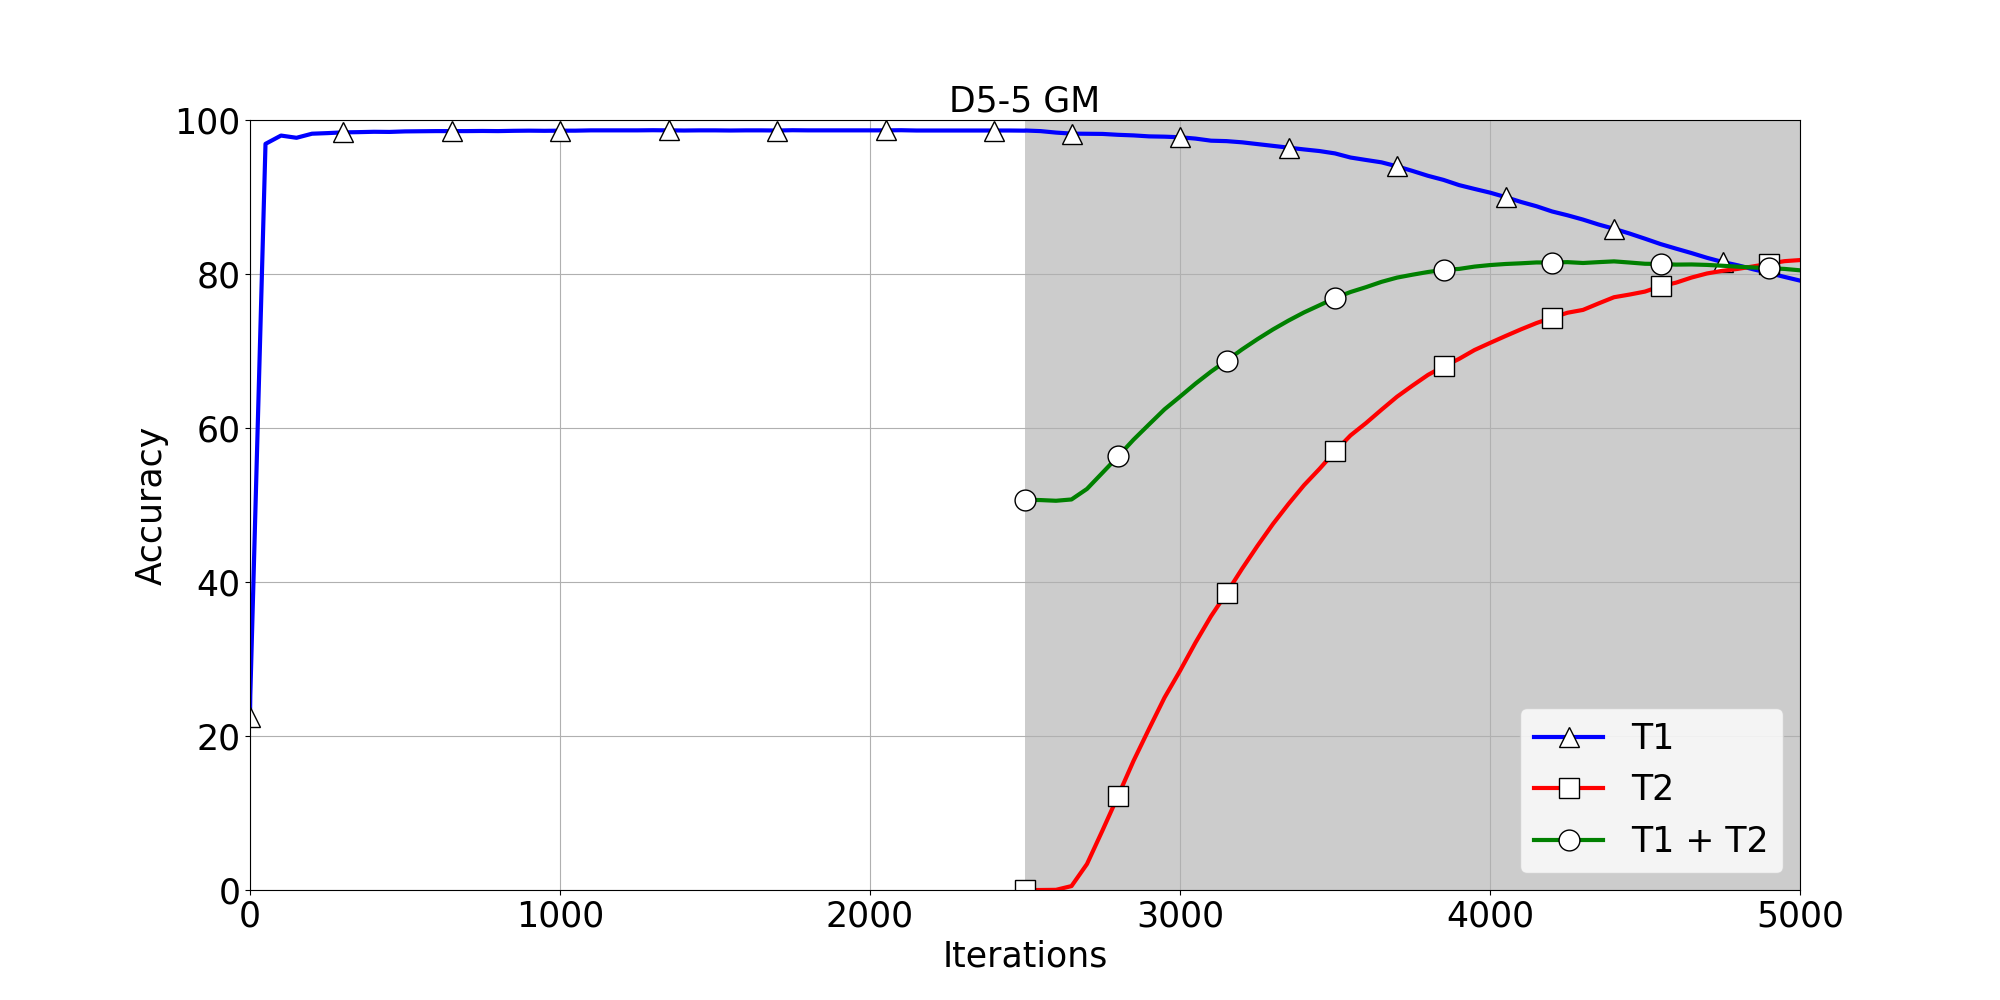
\includegraphics[width=\textwidth]{project/experiments/D55_GM}
    \caption{Experiment D5-5}
    \label{fig:exp_d5-5_bs1k}
\end{figure}

Figure \ref{fig:exp_d5-5_bs1k} shows the training of task $T_1$ (white background) and re-training with task $T_2$ (gray background).
The blue line ($\triangle$) represents the accuracy on $T_1$, the red line ($\square$) on $T_2$ and the green line ($\bigcirc$) the complete dataset ($T_1 + T_2$).
After the training, $T_1$ results in 99\% accuracy.
While re-training, the complete dataset increases its accuracy from 51\% to 80\%.
At the end of the re-training, $T_1$ is decreased to 79\% and $T_2$ measures 82\% accuracy.
It shows that the \acrshort{ewc} algorithm with the Gradient matrix reduces catastrophic forgetting in the re-training of an approximately equally task.

\begin{table}[H]
    \centering
    \begin{tabular}{ |c|l|l|l| }
        \hline
        \multicolumn{2}{|c|}{parameters} & \multicolumn{2}{c|}{accuracy} \\
        \hline
        learning rate & lambda & $T_2$ & complete dataset\\
        \hline
        \hline
        \multirow{6}{*}{0.001} & 1,000 & 97.87\% & 48.94\%\\
                            & 10,000 & 98.13\% & 49.84\%\\
                            & 100,000 & 97.94\% & 51.04\% \\
                            & 1,000,000 & 97.5\% & 51.72\% \\
                            & 1,010,000 & 97.27\% & 51.99\% \\
                            & 1,050,000 & 97.52\% & 52.75\% \\
        \hline
        \multirow{6}{*}{0.0001} & 1,000 & 97.05\% & 63.24\%\\
                                & 10,000 & 96.65\% & 63.49\%\\
                                & 100,000 & 96.19\% & 61.74\% \\
                                & 1,000,000 & 95.65\% & 63.14\% \\
                                & 1,010,000 & 95.74\% & 63.06\% \\
                                & 1,050,000 & 95.59\% & 63.03\% \\
        \hline
        \multirow{6}{*}{0.00001} & 1,000 & 93.64\% & 81.87\%\\
                                & 10,000 & 90.45\% & 83.49\%\\
                                & 100,000 & 82.38\% & 79.86\% \\
                                & 1,000,000 & 67.84\% & 72.68\% \\
                                & 1,010,000 & 67.79\% & 72.64\% \\
                                & 1,050,000 & 67.2\% & 72.42\% \\
        \hline
        \multirow{6}{*}{0.000001} & 1,000 & 28.1\% & 63.55\% \\
                                & 10,000 & 18.9\% & 59.39\% \\
                                & 100,000 & 0.02\% & 50.6\% \\
                                & 1,000,000 & 0.0\% & 50.71\% \\
                                & 1,010,000 & 0.0\% & 50.71\% \\
                                & 1,050,000 & 0.0\% & 50.71\% \\
        \hline
    \end{tabular}
    \caption{Experiment D5-5}
    \label{table:exp_d5-5}
\end{table}

Table \ref{table:exp_d5-5} summarizes several parameter tests based on Table \ref{table:exp_d55_params}.
It lists the end accuracy on $T_2$ as well as the complete dataset ($T_1 + T_2$) after the re-training.
\newline
A learning rate of 0.00001 and lambda value of 1,000 delivers the best incremental learning quality.
$T_2$ measures 94\% accuracy and the complete dataset results in 81\%.

\newpage

\subsection{Permuted 10-10}

This experiment uses the complete MNIST dataset in the training of task $T_1$ and permutes the complete dataset for the re-training with task $T_2$.
\newline
The training of the tasks $T_1$ and $T_2$ is implemented with the following hyperparameters:

\begin{table}[H]
    \centering
    \begin{tabular}{ |l|l|l| }
        \hline
        Task $\to$ & $T_1$ & $T_2$ \\
        \hline\hline
        samples & 60,000 & 60,000 \\
        \hline
        permutation seed & - & 0 \\
        \hline
        batch size & 100 & 100 \\
        \hline
        training iterations & 2,500 & 20,000 \\
        \hline
        learning rate & 0.001 & 0.00001 \\
        \hline
        \acrshort{gm} batch size & 1,000 & - \\
        \hline
        lambda ($\lambda$) & 0 & 100,000 \\
        \hline
    \end{tabular}
    \caption{Experiment P10-10 parameters}
    \label{table:exp_p1010_params}
\end{table}

\begin{figure}[H]
    \centering
    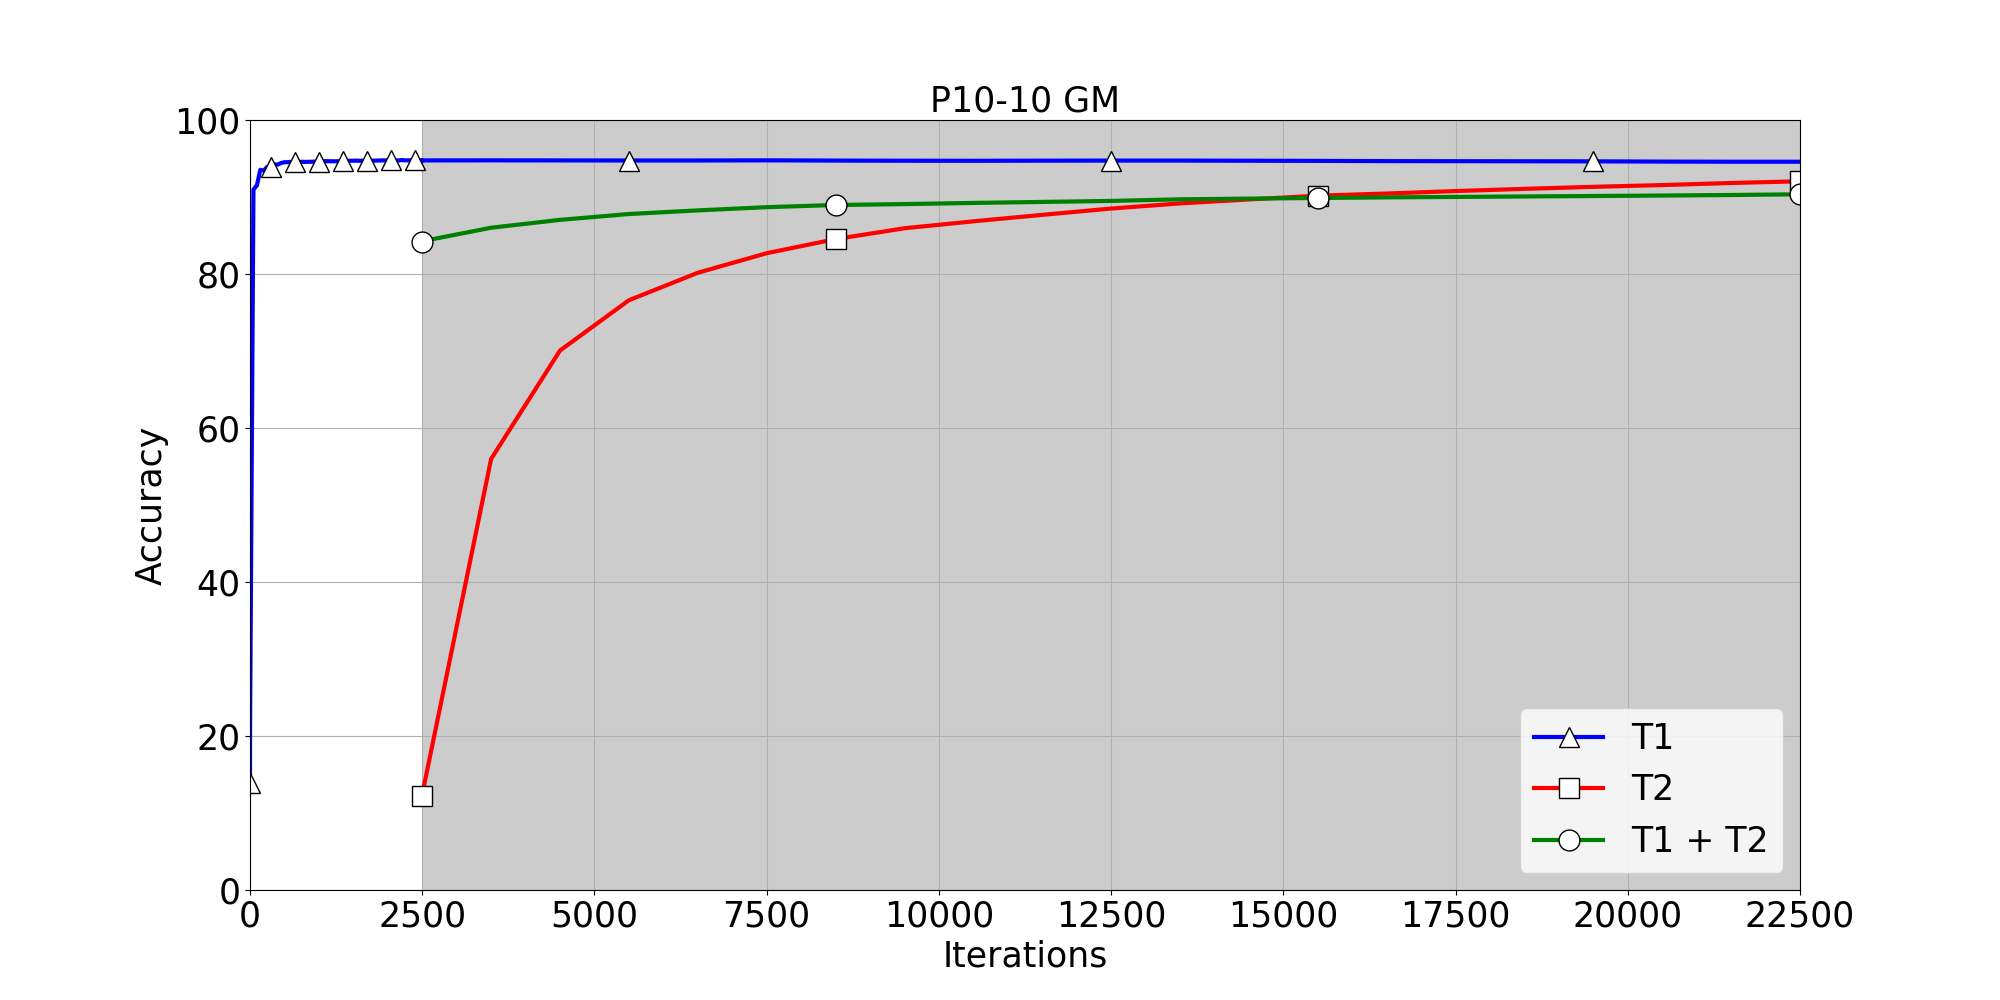
\includegraphics[width=\textwidth]{project/experiments/PM_GM}
    \caption{Experiment P10-10}
    \label{fig:exp_p10-10}
\end{figure}

Figure \ref{fig:exp_p10-10} shows the training of task $T_1$ (white background) and re-training with task $T_2$ (gray background).
The blue line ($\triangle$) represents the accuracy on $T_1$, the red line ($\square$) on $T_2$ and the green line ($\bigcirc$) the complete dataset ($T_1 + T_2$).
After the training, $T_1$ results in 95\% accuracy.
The complete dataset starts with 84\% accuracy into the re-training.
It is able to gain 6\% and quantifies 90\% accuracy at the end of the re-training.
$T_1$ still measures 95\% accuracy and $T_2$ amounts 92\% accuracy.
\newline
The challenge of learning different data with the same output classes turns out to be feasible.

\begin{table}[H]
    \centering
    \begin{tabular}{ |c|l|l|l|  }
        \hline
        \multicolumn{2}{|c|}{parameters} & \multicolumn{2}{c|}{accuracy} \\
        \hline
        learning rate & lambda & $T_2$ & complete dataset\\
        \hline
        \hline
        \multirow{6}{*}{0.001} & 1,000 & 97.09\% & 93.72\%\\
                            & 10,000 & 97.66\% & 94.20\%\\
                            & 100,000 & 97.2\% & 93.05\% \\
                            & 1,000,000 & 97.3\% & 93.26\% \\
                            & 1,010,000 & 97.25\% & 92.46\% \\
                            & 1,050,000 & 96.84\% & 92.29\% \\
        \hline
        \multirow{6}{*}{0.0001} & 1,000 & 96.87\% & 91.41\%\\
                                & 10,000 & 96.51\% & 90.93\%\\
                                & 100,000 & 96.48\% & 91.45\% \\
                                & 1,000,000 & 96.45\% & 91.47\% \\
                                & 1,010,000 & 96.56\% & 91.43\% \\
                                & 1,050,000 & 96.45\% & 91.38\% \\
        \hline
        \multirow{6}{*}{0.00001} & 1,000 & 94.67\% & 90.98\%\\
                                & 10,000 & 93.04\% & 90.67\%\\
                                & 100,000 & 91.53\% & 90.46\% \\
                                & 1,000,000 & 90.29\% & 90.66\% \\
                                & 1,010,000 & 90.28\% & 90.65\% \\
                                & 1,050,000 & 90.23\% & 90.66\% \\
        \hline
        \multirow{6}{*}{0.000001} & 1,000 & 87.84\% & 89.75\% \\
                                & 10,000 & 80.58\% & 89.67\% \\
                                & 100,000 & 68.64\% & 89.17\% \\
                                & 1,000,000 & 56.66\% & 88.64\% \\
                                & 1,010,000 & 56.62\% & 88.63\% \\
                                & 1,050,000 & 56.51\% & 88.62\% \\
        \hline
    \end{tabular}
    \caption{Experiment P10-10}
    \label{table:exp_p10-10}
\end{table}

Table \ref{table:exp_p10-10} summarizes several parameter tests based on Table \ref{table:exp_p1010_params}.
It lists the end accuracy on $T_2$ and the complete dataset ($T_1 + T_2$) after the re-training.
\newline
Many parameter combinations offer promising results.
Nevertheless, the combination of a small learning rate and a small lambda value outperform higher parameter values.
